En esta seccion se documenta la arquitectura logica actual del sistema, centrada en la aplicacion web, la organizacion del codigo y las integraciones externas necesarias para soportar los modulos ya implementados, incluido \texttt{M4}.

\subsection{Diseno de alto nivel}

KinEstilistas se implementa como una aplicacion web monolitica full-stack. La misma base de codigo contiene tanto la interfaz de usuario como la logica de servidor y el acceso a datos, lo que simplifica la trazabilidad entre requisitos, codigo y despliegue.

Los contenedores logicos que forman la solucion son los siguientes:

\begin{itemize}
    \item \textbf{Cliente web}: interfaz renderizada con \texttt{Next.js} y \texttt{React}, diferenciada por rol.
    \item \textbf{Servidor de aplicacion}: \texttt{Route Handlers}, autenticacion, proteccion de rutas, validacion y orquestacion de servicios.
    \item \textbf{Base de datos relacional}: \texttt{PostgreSQL}, persistida y versionada mediante migraciones.
    \item \textbf{Servicios externos}: \texttt{Cloudinary} para imagenes, \texttt{Nominatim} para geocodificacion, \texttt{OSRM} para trazado de rutas y \texttt{QuickChart} para la representacion del QR operativo de pedido.
\end{itemize}

La aplicacion resuelve ademas varias responsabilidades transversales desde una capa comun:

\begin{itemize}
    \item autenticacion y sesion con \texttt{Auth.js},
    \item control de acceso por rol,
    \item compatibilidad minima de navegador,
    \item rate limiting sobre \texttt{/api},
    \item contratos de datos compartidos entre cliente y servidor.
\end{itemize}

\subsection{Diseno detallado}

La estructura del codigo combina una organizacion por capas tecnicas con subdirectorios funcionales para las areas principales del dominio.

\begin{itemize}
    \item \texttt{app/admin/}, \texttt{app/commercials/} y \texttt{app/clients/}: entrada funcional por rol.
    \item \texttt{app/api/}: endpoints internos segmentados por area de negocio.
    \item \texttt{app/components/}: componentes de interfaz reutilizables, incluyendo formularios, mapas, tablas y vistas especializadas de pedido o reparto.
    \item \texttt{app/hooks/api/}: capa cliente para acceso declarativo a la API.
    \item \texttt{lib/contracts/}: DTOs y contratos comunes.
    \item \texttt{lib/commercial/}: logica de planificacion de rutas y calculo temporal reutilizable.
    \item \texttt{lib/clients/}: lectura de ETA y resumen de reparto para la zona cliente.
    \item \texttt{lib/orders/}: utilidades operativas del dominio de pedidos, como el soporte QR.
    \item \texttt{lib/typeorm/entities/} y \texttt{lib/typeorm/services/}: modelo persistente y servicios de dominio asociados a la base de datos.
    \item \texttt{migrations/typeorm/}: evolucion versionada del esquema.
\end{itemize}

\paragraph{Flujo tipico de una operacion protegida}

El flujo interno de una operacion sensible sigue de forma general los siguientes pasos:

\begin{enumerate}
    \item La peticion llega a \texttt{proxy.ts}, donde se aplica control de navegador, autenticacion base y rate limiting.
    \item La pagina o el endpoint correspondiente obtiene la sesion y comprueba el rol requerido.
    \item El \textit{Route Handler} delega la logica de negocio en servicios o helpers de \texttt{lib/}.
    \item Si se requiere persistencia, la operacion utiliza \texttt{TypeORM} sobre entidades y repositorios.
    \item La respuesta se normaliza y se devuelve al cliente mediante contratos compartidos.
\end{enumerate}

\paragraph{Organizacion actual por carpetas}

La arquitectura de carpetas actual es adecuada para el alcance ya construido, porque separa claramente:

\begin{itemize}
    \item vistas por rol,
    \item componentes visuales reutilizables,
    \item integraciones externas,
    \item persistencia y migraciones.
\end{itemize}

No obstante, el crecimiento conjunto de los modulos comercial y de pedidos ya apunta a una evolucion deseable: reforzar la agrupacion por \textit{feature} para reducir la dispersion entre componentes, hooks, contratos y servicios relacionados con una misma capacidad de negocio. La base actual sigue siendo valida, pero esta mejora seria especialmente interesante en futuras iteraciones del flujo completo de \texttt{M2} y \texttt{M4}.

\subsection{Gestion de almacenamiento de imagenes de perfil}
\label{sec:storageDesign}
En el estado actual del proyecto, el \textbf{almacenamiento del sistema} se divide en tres categorías complementarias: \textbf{datos estructurados persistentes}, \textbf{activos multimedia externos} y \textbf{datos operativos derivados} bajo demanda.

\subsubsection*{Datos estructurados persistentes}

La \textbf{información principal del dominio} se almacena en \texttt{PostgreSQL} mediante entidades gestionadas con \texttt{TypeORM}. Esto incluye:

\begin{itemize}
    \item \textbf{Usuarios}, solicitudes de alta, accesos y trazabilidad administrativa;
    \item \textbf{Clientes}, comerciales y asignaciones entre ambos;
    \item \textbf{Visitas}, rutas comerciales y ordenación de paradas;
    \item \textbf{Catálogo}, productos, cartas de color y referencias cromáticas;
    \item \textbf{Pedidos}, líneas de pedido, repartos, líneas de reparto, estados de negocio, pagos parciales y estado de cobro derivado;
    \item \textbf{Fichas técnicas del salón}, servicios, plantillas, productos utilizados, sugerencias e imágenes finales referenciadas;
    \item \textbf{Segmentos de cliente}, asignaciones comerciales de segmentación, promociones, formaciones, inscripciones, notificaciones internas, recordatorios y suscripciones \textit{Web Push} de usuario;
    \item \textbf{Catálogos controlados} de roles, estados y tipos operativos utilizados por los módulos ya implementados;
    \item Sobrescrituras técnicas persistidas para políticas de \textit{rate limiting};
    \item Configuraciones del sistema, tarifa de agencia, integraciones externas, operaciones de integración y propuestas de pedido a proveedor con sus líneas.
\end{itemize}

Este modelo relacional actúa como \textbf{fuente de verdad del sistema}. Las operaciones críticas de autenticación, gestión comercial, catálogo, pedidos, administración transversal y operación empresarial se apoyan en esta capa. La Figura~\ref{fig:postgresql-physical-model} resume el \textbf{diseño físico de PostgreSQL} agrupando las tablas reales por módulo funcional y mostrando las dependencias principales entre áreas. Las relaciones internas con mayor detalle quedan documentadas en los modelos conceptuales de datos y en las migraciones de \texttt{TypeORM}.

\begin{figure}[p]
    \centering
    \rotatebox{90}{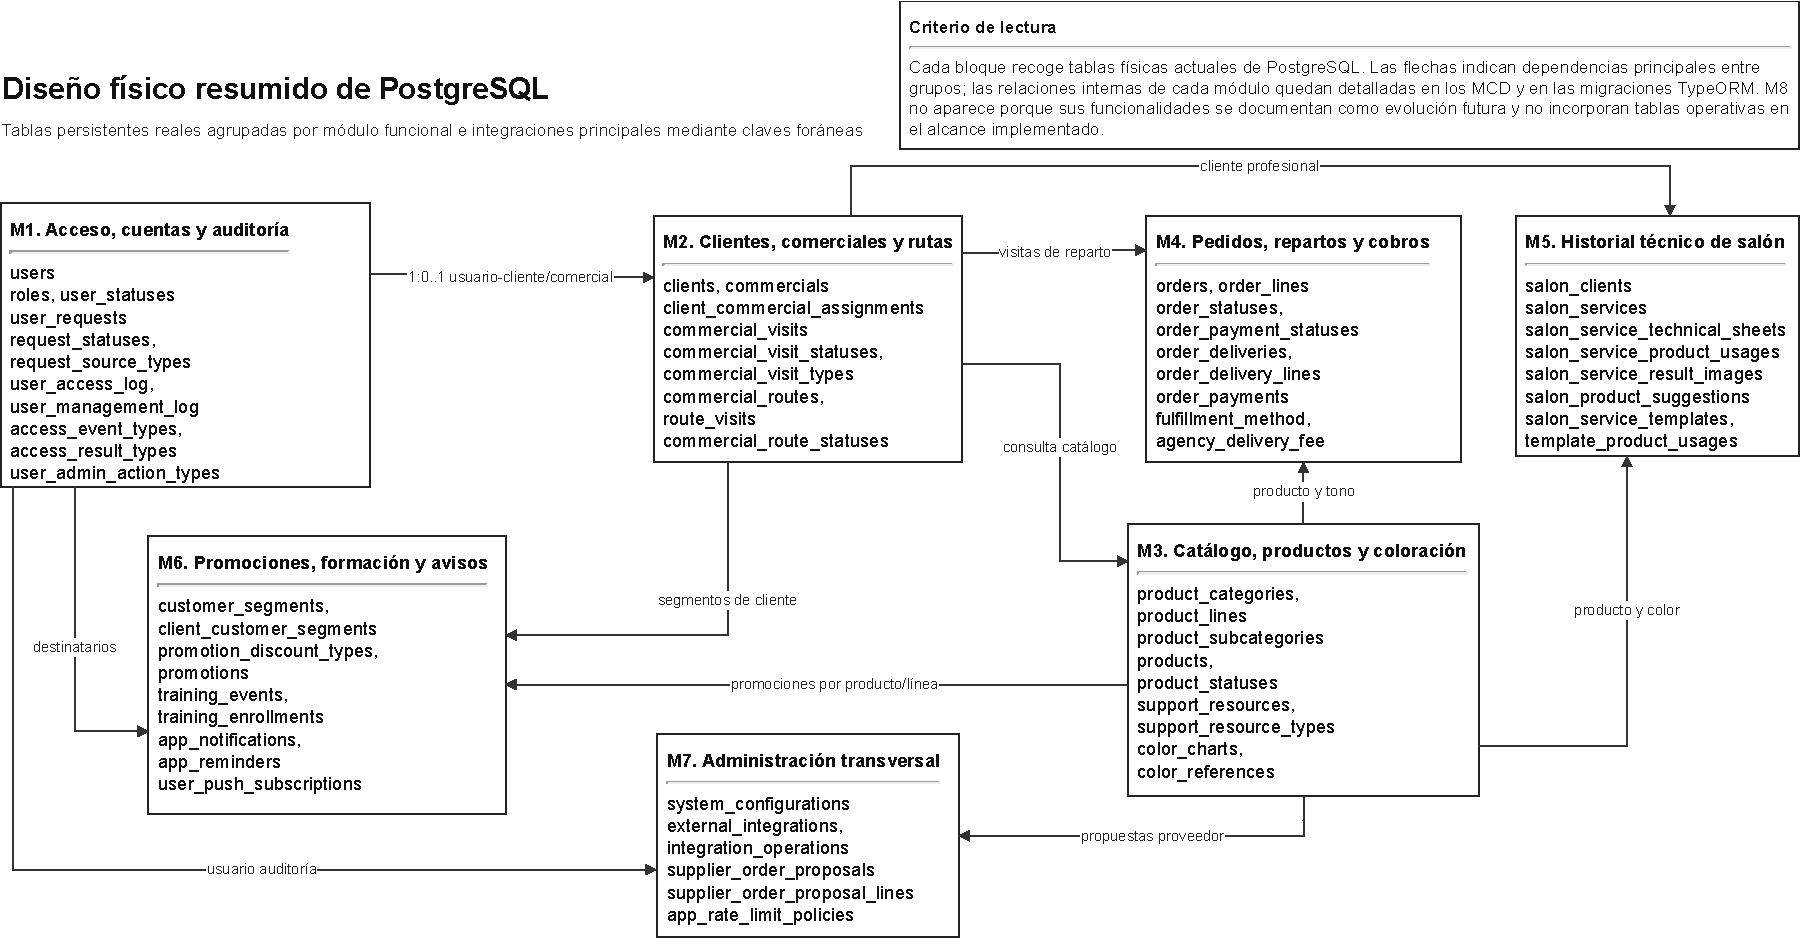
\includegraphics[width=0.92\textheight,height=0.98\textwidth,keepaspectratio]{./figures/UML/MCD/postgresql-physical-model.pdf}}
    \caption{Vista física resumida del modelo relacional de PostgreSQL}
    \label{fig:postgresql-physical-model}
\end{figure}

\subsubsection*{Activos multimedia externos}

Las \textbf{imágenes y documentos} subidos desde la aplicación no se almacenan como binarios en la base de datos. En su lugar, la aplicación delega su gestión en \texttt{Cloudinary}. Esta decisión afecta actualmente a cinco familias de activos:

\begin{itemize}
    \item \textbf{Imágenes de perfil} de usuarios;
    \item \textbf{Imágenes de catálogo}, incluyendo líneas, subcategorías, productos, cartas de color y referencias cromáticas;
    \item \textbf{Imágenes del resultado final} de servicios técnicos registrados en el salón;
    \item \textbf{Documentos y recursos de apoyo} del catálogo, como fichas o materiales asociados;
    \item \textbf{Adjuntos de promociones}, tanto imágenes comerciales como documentos \textit{PDF}.
\end{itemize}

En la base de datos solo se persisten las \textbf{URLs finales} y, cuando procede, metadatos auxiliares como la miniatura asociada a una referencia cromática, el tipo de recurso o la relación funcional con producto, promoción o servicio técnico. Esto simplifica el modelo, reduce el peso de la base de datos y permite reutilizar un almacenamiento optimizado para contenido multimedia y documental.

La \textbf{elección de \texttt{Cloudinary}} se debe a que el proyecto necesita almacenar y servir imágenes desde una aplicación web desplegable en entornos donde el sistema de ficheros local no debe considerarse persistente. Se descartó guardar binarios directamente en \texttt{PostgreSQL}, ya que aumentaría el tamaño de la base de datos, complicaría copias de seguridad y mezclaría datos transaccionales con recursos pesados. También sería posible utilizar alternativas como almacenamiento de objetos genérico, pero \texttt{Cloudinary} ofrece de forma directa subida, alojamiento, URLs públicas y gestión orientada a imágenes, lo que reduce el esfuerzo de integración dentro del alcance del TFG \citep{cloudinaryupload2026}.

Desde el punto de vista económico, \texttt{Cloudinary} \textbf{no se asume como gratuito de forma indefinida}. Para la demostración y una primera operación de baja carga se contempla el plan gratuito dentro de la estimación base; si el catálogo, los adjuntos o el consumo de ancho de banda superasen esos límites, el coste pasaría a formar parte de la operación del sistema y debería ser asumido por la entidad que mantenga la aplicación en producción, tal como se refleja en la estimación de infraestructura de la Tabla~\ref{tabla_coste_infraestructura} \citep{cloudinarypricing2026}.

\subsubsection*{Datos derivados o reconstruibles}

Existen además varios \textbf{artefactos derivados o reconstruibles} que la aplicación no persiste como entidad independiente:

\begin{itemize}
    \item El \textit{QR} del reparto comercial, que se reconstruye a partir del identificador del reparto y se representa mediante \texttt{QuickChart} \citep{quickchartqr2026};
    \item La etiqueta de agencia, que reutiliza el mismo formato de etiqueta logística pero sustituye el bloque QR por una marca textual de agencia;
    \item La geometría de ruta comercial, que se consulta a \texttt{OSRM} cuando debe recalcularse la planificación diaria \citep{osrmdocs2026};
    \item La geocodificación de una dirección, que se obtiene desde \texttt{Nominatim} cuando hace falta confirmar o recalcular coordenadas \citep{nominatimapi2026};
    \item La \textit{ETA} visible para cliente, que se obtiene a partir de visitas reales, reglas horarias y posición en ruta, persistiendo los resultados operativos de llegada y salida cuando la planificación diaria se recalcula;
    \item Los envíos externos de comunicaciones, que pueden emitirse por correo SMTP o \textit{Web Push} a partir de una notificación interna persistida; si la integración no está configurada, la notificación interna se conserva como canal principal.
\end{itemize}

Esta separación evita almacenar \textbf{resultados efímeros o fácilmente regenerables} cuando su valor depende de datos del negocio ya presentes en el sistema.

En el caso del \textit{QR}, se utiliza \texttt{QuickChart} porque el sistema solo necesita obtener una \textbf{representación visual estable} a partir de un identificador de reparto. Persistir una imagen \textit{QR} por cada reparto o incorporar una librería adicional de renderizado en la interfaz habría añadido almacenamiento o dependencia cliente sin aportar trazabilidad adicional. Con esta solución, el dato relevante sigue siendo el identificador persistido del reparto, mientras que la imagen se regenera cuando hace falta. Al igual que con el resto de servicios externos, el coste base considerado es nulo para una primera implantación de bajo volumen, pero el paso a un plan de pago quedaría como coste operativo si se superasen los límites del plan comunitario documentado en la Tabla~\ref{tabla_coste_infraestructura} \citep{quickchartqr2026,quickchartpricing2026}.

\subsubsection*{Criterios de diseño adoptados}

La \textbf{estrategia de almacenamiento} aplicada en el proyecto responde a cuatro criterios:

\begin{itemize}
    \item Mantener el \textbf{dato estructurado y transaccional} dentro de la base de datos relacional;
    \item Externalizar los \textbf{binarios y recursos multimedia} a un servicio especializado;
    \item Recalcular bajo demanda la \textbf{información derivada} cuando sea más robusto que persistirla;
    \item Limitar el número de entidades persistentes a las que realmente aportan valor al modelo de negocio implementado.
\end{itemize}

Por ello, aunque el sistema ya muestra \textit{QR}, \textit{ETA}, mapas, capturas de cámara o recursos externos, no todo ello debe interpretarse como nuevas entidades almacenadas. La memoria debe distinguir entre \textbf{datos persistidos}, \textbf{activos referenciados} e \textbf{información operativa calculada} o regenerada a partir de datos persistentes.
